\begin{problem}
  Evaluate each of the following expressions; provide exact values. Be
  sure to use proper notation to communicate your answers, i.e., link the
  given expressions and your answers with equal signs. An example has been
  provided to clarify how your responses should be organized. \textbf{[$15$ points]}

    \begin{enumerate}
      \item Evaluate $\cos \left(\frac{\pi}{3}\right)$ \textbf{[$1$ point]}

        \begin{align*}
          \cos \left(\frac{\pi}{3}\right) = \frac{1}{2}
        .\end{align*}

      \item Evaluate $\sin \left(\frac{5\pi}{6}\right)$ \textbf{[$1$ point]}

        \begin{align*}
          \sin \left(\frac{5\pi}{6}\right) = \frac{1}{2} \\
        .\end{align*}

      \item Evaluate $\cos (210^{\circ})$ \textbf{[$1$ point]}

        \begin{align*}
          \cos (210^{\circ}) = -\frac{\sqrt{3}}{2}
        .\end{align*}

      \item Evaluate $\csc (60^{\circ})$ \textbf{[$1$ point]}

        \begin{align*}
          \csc (60^{\circ}) &= \frac{1}{\sin (60^{\circ})} \\
                            &= \frac{1}{\frac{\sqrt{3}}{2}} = \frac{2\sqrt{3}}{3} \\
        .\end{align*}

      \item Evaluate $\sec \left(\frac{11\pi}{6}\right)$ \textbf{[$1$ point]}

        \begin{align*}
          \sec \left(\frac{11\pi}{6}\right) &= \frac{1}{\cos \left(\frac{11\pi}{6}\right)} \\
                                            &= \frac{1}{\frac{\sqrt{3}}{2}} = \frac{2\sqrt{3}}{3} \\
        .\end{align*}

      \item Evaluate $\tan \left(\frac{5\pi}{4}\right)$ \textbf{[$1$ point]}

        \begin{align*}
          \tan \left(\frac{5\pi}{4}\right) &= \frac{\sin \left(\frac{5\pi}{4}\right)}{\cos \left(\frac{5\pi}{4}\right)} \\
                                           &= \frac{\frac{\sqrt{2}}{-2}}{\frac{\sqrt{2}}{-2}} = 1
        .\end{align*}
    \end{enumerate}
\end{problem}

\newpage

\begin{problem}
  The point $A$ in Figure 1 is specified by $\frac{7\pi}{6}$ on the
  circumference of a circle of radius $8$ units. Use the sin and cos functions
  to find the \textbf{exact} coordinates of point $A$. \textbf{[Be sure to
  \textit{show} your use of sin and cos.]} \textbf{[$3$ points]}

  \begin{figure}[htpb]
    \centering
    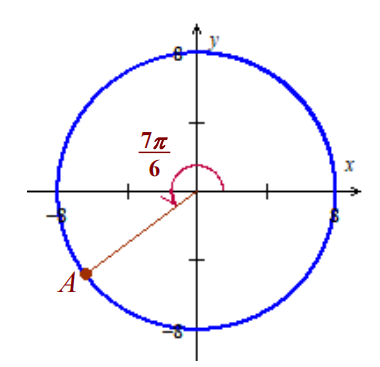
\includegraphics[width=0.8\textwidth]{images/week-2.png}
    \caption{}
    \label{fig:}
  \end{figure}

  \begin{align*}
    \sin \left(\frac{7\pi}{6}\right) &= -\frac{1}{2} \\
    \cos \left(\frac{7\pi}{6}\right) &= -\frac{\sqrt{3}}{2}
  .\end{align*}

  So, the exact coordinates of point $A$ are:
  \[ \left(\frac{\sqrt{3}}{2}, -\frac{1}{2}\right) \].
\end{problem}

\newpage

\begin{problem}
  If $\sin (A) = \frac{5}{6}$ and $\frac{\pi}{2} < A < \pi$ (i.e., angle $A$ is
  in the second quadrant), find the following \textbf{without using any inverse
  functions}. (Provide \textbf{exact} completely simplified numerical answers;
  as shown above in the example given in \#1, use proper notation to
  \textbf{directly communicate} what given expressions equal.) \textbf{[$6$ points]}

  \begin{align*}
    &y = 5 \\
    &r = 6 \\
    &x = x^{2} + 5^{2} = 6^{2} \implies -\sqrt{11} \\
  .\end{align*}

  \begin{enumerate}
    \item $\cos (A)$ \textbf{[$3$ points]}
      \[ \cos = -\frac{\sqrt{11}}{6} \].
    \item $\tan (A)$ \textbf{[$1.5$ points]}
      \[ \tan (A) = \frac{\sin (A)}{\cos (A)} = -\frac{5}{\sqrt{11}} \].
    \item $\csc (A)$ \textbf{[$1.5$ points]}
      \[ \csc (A) = \frac{1}{\sin (A)} = \csc (A) = \frac{5}{2} \].
  \end{enumerate}
\end{problem}
